\documentclass[UTF8]{ctexart}
\usepackage{amsmath}
\usepackage{diagbox}
\usepackage{textcomp}
\usepackage{graphicx}
\usepackage{float}
\usepackage{caption}
\usepackage{adjustbox}
\usepackage{subfigure}
\usepackage{geometry}
\usepackage{pifont}
\usepackage{bm}
\begin{document}
\renewcommand{\thefootnote}{\fnsymbol{footnote}}
\newgeometry{left=2cm,bottom=4cm,right=2cm}
%\pagestyle{plain}
\linespread{1.4}
\title{\vspace{-5em}\heiti几何光学实验报告\vspace{-2.5em}}
\date{}
\maketitle
\begin{center}
{\fangsong 徐浩博\quad 基科01\quad2020010108}
\end{center}

\subsubsection*{摘要}
{\kaishu\normalsize  本实验旨在通过透镜在不同条件下成像的观察、测量与分析,使我掌握了透镜成像的基本规律,知晓了主面主点等相关概念,了解了进行几何光学实验的一些基本要求和注意事项,掌握了几种常见的测量凸/凹透镜焦距的方法,并使我对一些基本的光学仪器如望远镜、显微镜成像原理产生了更深刻的理解. 同时,通过各种曲线的绘制,我还掌握了图线绘制和测量的基本操作和方法,掌握了相关软件的使用方法,并再一次巩固了误差分析和不确定度计算等相关知识.}
\subsubsection*{关键词:\quad几何光学\quad透镜成像\quad共轴调节\quad焦距\quad主面间距\quad理想透镜组\quad内调焦望远镜\quad \vspace{1.5em}}


\section{实验仪器}
1.8米光学导轨\par
凸透镜(复合透镜、长焦透镜各一)、凹透镜\par
光源、物屏、像屏、平行光管\par
测微目镜、读数显微镜\par

\section{实验原理及实验数据}

\subsection*{ A) 共轴调节}
我们近似认为平行光管和光学导轨水平,进行实验时仍需将其他的光学仪器调整于水平面上,下面是具体步骤:\par
1. 粗调,将物(平行光管/物屏)、单个凸透镜、像(像屏/测微目镜/读数显微镜)靠拢,目测调节高低左右,使三者近似平行于水平导轨.\par
2. 粗测,估测凸透镜焦距. 在这里我们可以采用三种方法: i)将太阳光透射到地面上,用直尺估计焦距; ii)利用物屏像屏测量一组物距像距,利用透镜成像公式估计焦距; iii)固定透镜位置,利用物屏像屏,将二者近似等距离同时拉远,屏上成清晰像时,物距像距大约等于2倍焦距,此时物像大小也近似相等.\par
3. 细调,采用大像追小像的方法,让物与像相距4倍凸透镜焦距以上,移动透镜过程中会成两次像,两次像的成像位置应大致相同,否则需要上下左右调整透镜或物.\par
4. 加置其他光学仪器. 透镜组成像时,需要在一个透镜调整完成后再一个个加置其他透镜,采用1-3的方法,调整过程中只调整该透镜的位置. 针对凹透镜,得需要调好一个凸透镜后才能安置凹透镜共轴调节.\par
注意,对于读数显微镜/测微目镜,我们只需在看清像后上下左右移动读数显微镜/测微目镜直到叉丝中心对准分划板线对中心即可.


\subsection*{ B) 薄凸透镜焦距的测量}
下面我们采用三种方法进行透镜焦距的测量. 我们采用物距像距法和和共轭法测量复合透镜,并对两个测量结果进行横向比较;最后,我们用焦距仪法测量长焦透镜,并进行不确定度的计算.\par
\subsubsection*{B.1 物距像距法测复合透镜焦距}
\paragraph{实验原理及操作如下:}\quad\par
我们将该透镜近似等效为薄透镜,设物距$l$,像距$l'$,焦距$f$,于是利用薄透镜成像公式:
\begin{equation}
    \frac{1}{l}+\frac{1}{l'}=\frac{1}{f}
\end{equation}
以此得到:
\begin{equation}
    \label{wujuxiangjufa}
    {f}=\frac{1}{\frac{1}{l}+\frac{1}{l'}}
\end{equation}
由该公式,我们只需测量一次成像的物距、像距即可得到焦距.\par
具体到实验操作,测量时先进行物屏、透镜、像屏的共轴调节. 然后固定物屏和透镜的位置,在透镜后方反复移动像屏寻找最清晰的像,成像最清晰时固定像屏,记录像、镜、物三者坐标分别为$z_I$、$z_L$、$z_O$,即可得到\textbf{物距}\bm{$l=z_O-z_L$}和\textbf{像距}\bm{$l'=z_l-z_I$},再由公式就可计算出透镜焦距. 需要注意的是,这里的物距指物屏中心与透镜光心之间的距离.\par
为了得到更精确的结果,我们进行多次测量,并保证测量条件分别满足$f<l<2f$、$l\approx 2f$、$l>2f$三种条件. \par
在正式实验之前,利用A)中提及的粗测方法对其焦距进行估计,得到焦距$f\approx 15cm$,以此控制条件来进行实验. \par

\paragraph{测量数据如下:}\quad\par
\begin{table}[H]\begin{center}
    \caption{物距像距法测凸透镜焦距测量数据表}
    \begin{tabular}{|c|c|c|c|c|c|c|}
        \hline
        组别&像屏坐标$z_I$/cm&透镜中心坐标$z_L$/cm&物屏坐标$z_O$/cm\\
        \hline
        1$(f<l<2f)$&10.12&60.00&82.50\\
        \hline
        2$(l\approx 2f)$&28.05&60.00&90.00\\
        \hline
        3$(l>2f)$&37.28&60.00&110.00\\
        \hline 
    \end{tabular}
\end{center}\end{table}
\paragraph{数据处理如下:}\quad\par
\paragraph{第一组$(f<l<2f)$}\quad
\begin{center}
    物距\quad$l_1=z_{O1}-z_{L1}=82.50cm-60.00cm=22.50cm$\\
    像距\quad$l'_1=z_{L1}-z_{I1}=60.00cm-10.12cm=49.88cm$\\
\end{center}
由(\ref{wujuxiangjufa})式得:\par
\begin{center}凸透镜焦距\quad
$\displaystyle{   
     {f'_{x1}}=\frac{1}{\frac{1}{l_1}+\frac{1}{l
    '_1}}=\frac{1}{\frac{1}{22.50cm}+\frac{1}{49.88cm}}=15.50cm
}$
\end{center}

\paragraph{第二组$(l\approx2f)$}\quad
\begin{center}
    物距\quad$l_2=z_{O2}-z_{L2}=90.00cm-60.00cm=30.00cm$\\
    像距\quad$l'_2=z_{L2}-z_{I2}=60.00cm-28.05cm=31.95cm$\\
\end{center}
由(\ref{wujuxiangjufa})式得:\par
\begin{center}凸透镜焦距\quad
$\displaystyle{   
     {f'_{x2}}=\frac{1}{\frac{1}{l_2}+\frac{1}{l'_2}}=\frac{1}{\frac{1}{30.00cm}+\frac{1}{31.95cm}}=15.47cm
}$
\end{center}

\paragraph{第三组$(l>2f)$}\quad
\begin{center}
    物距\quad$l_3=z_{O3}-z_{L3}=110.00cm-60.00cm=50.00cm$\\
    像距\quad$l'_3=z_{L3}-z_{I3}=60.00cm-37.28cm=22.72cm$\\
\end{center}
由(\ref{wujuxiangjufa})式得:\par
\begin{center}凸透镜焦距\quad
$\displaystyle{   
     {f'_{x3}}=\frac{1}{\frac{1}{l_3}+\frac{1}{l'_3}}=\frac{1}{\frac{1}{50.00cm}+\frac{1}{22.72cm}}=15.62cm
}$
\end{center}
观察以上的计算结果,凸透镜测量值偏差不大,说明实验方法和数据测量、计算基本正确,计算出焦距平均值:
\[f_1=\frac{f'_{x1}+f'_{x2}+f'_{x3}}{3}=\frac{15.50cm+15.47cm+15.62cm}{3}=15.53cm\]

\subsubsection*{B.2 共轭法测凸透镜焦距}
\paragraph{实验原理及操作如下:}\quad\par
理想透镜成像时,当物、像相距$4f$以上,则固定物屏、像屏而改变透镜位置,像屏上会成两次像. 根据光路可逆原理,两次成像时透镜关于物像之间的中点对称,设第一次物距像距分别为$l$与$l'$(不妨设l>l'),则第二次分别为$l'$与$l$,记$a=l-l'$,$b=l+l'$,则由(\ref{wujuxiangjufa})式得:
\begin{equation}
    \label{gongefa}
    f=\frac{1}{\frac{1}{l}+\frac{1}{l'}}=\frac{ll'}{l+l'}=\frac{b^2-a^2}{4b}
\end{equation}
实验时,固定物、像位置,测量两次成像透镜中心坐标$z_{L1}$、$z_{L2}$、成像时物坐标$z_O$、像坐标$z_I$,即可计算出$a=\big{|}z_{L1}-z_{L2}\big{|}$、$b=\big{|}z_{O}-z_{I}\big{|}$,便可以通过公式得到透镜焦距. \par注意,为了使两次成像时透镜位置间距稍远以减小误差,我们取物像间距$b=l+l'>5f'$,这里的$f'$可以根据估测或者B.2计算得出.\par

\paragraph{测量数据如下:}\quad\par
\begin{table}[H]\begin{center}
    \caption{共轭法测凸透镜焦距测量数据表}
    \begin{tabular}{|c|c|c|c|}
        \hline
        像屏坐标$z_I$/cm&物屏坐标$z_O$/cm&第一次成像透镜坐标$z_{L1}$/cm&第二次成像透镜坐标$z_{L2}$/cm\\
        \hline
        20.00&110.00&40.16&89.95\\
        \hline
    \end{tabular}
\end{center}\end{table}
\paragraph{数据处理如下:}\quad\par
\begin{center}
    共轭点间距\quad$a=\big{|}z_{L1}-z_{L2}\big{|}=\big{|}89.95cm-40.16cm\big{|}=49.79cm$\\
    物像间距\quad$b=\big{|}z_{O}-z_{I}\big{|}=\big{|}110.00cm-20.00cm\big{|}=90.00cm$
\end{center}
由(\ref{gongefa})式得:
\begin{center}
    透镜焦距\quad$\displaystyle{f=\frac{b^2-a^2}{4b}=\frac{90.00^2-49.79^2}{4\times 90.00}cm=15.61cm}$
\end{center}
对比B.1,B.2的实验结果,考虑到此实验具有将厚透镜等效为薄透镜等一系列误差,而二者实验结果十分接近,则基本验证了实验原理及操作过程的正确性.                                                

\subsubsection*{B.3 焦距仪法测凸透镜焦距}
\paragraph{实验原理及操作如下:}\quad\par
下图为成像时的光路图:
\begin{figure}[H]
    \begin{center}
    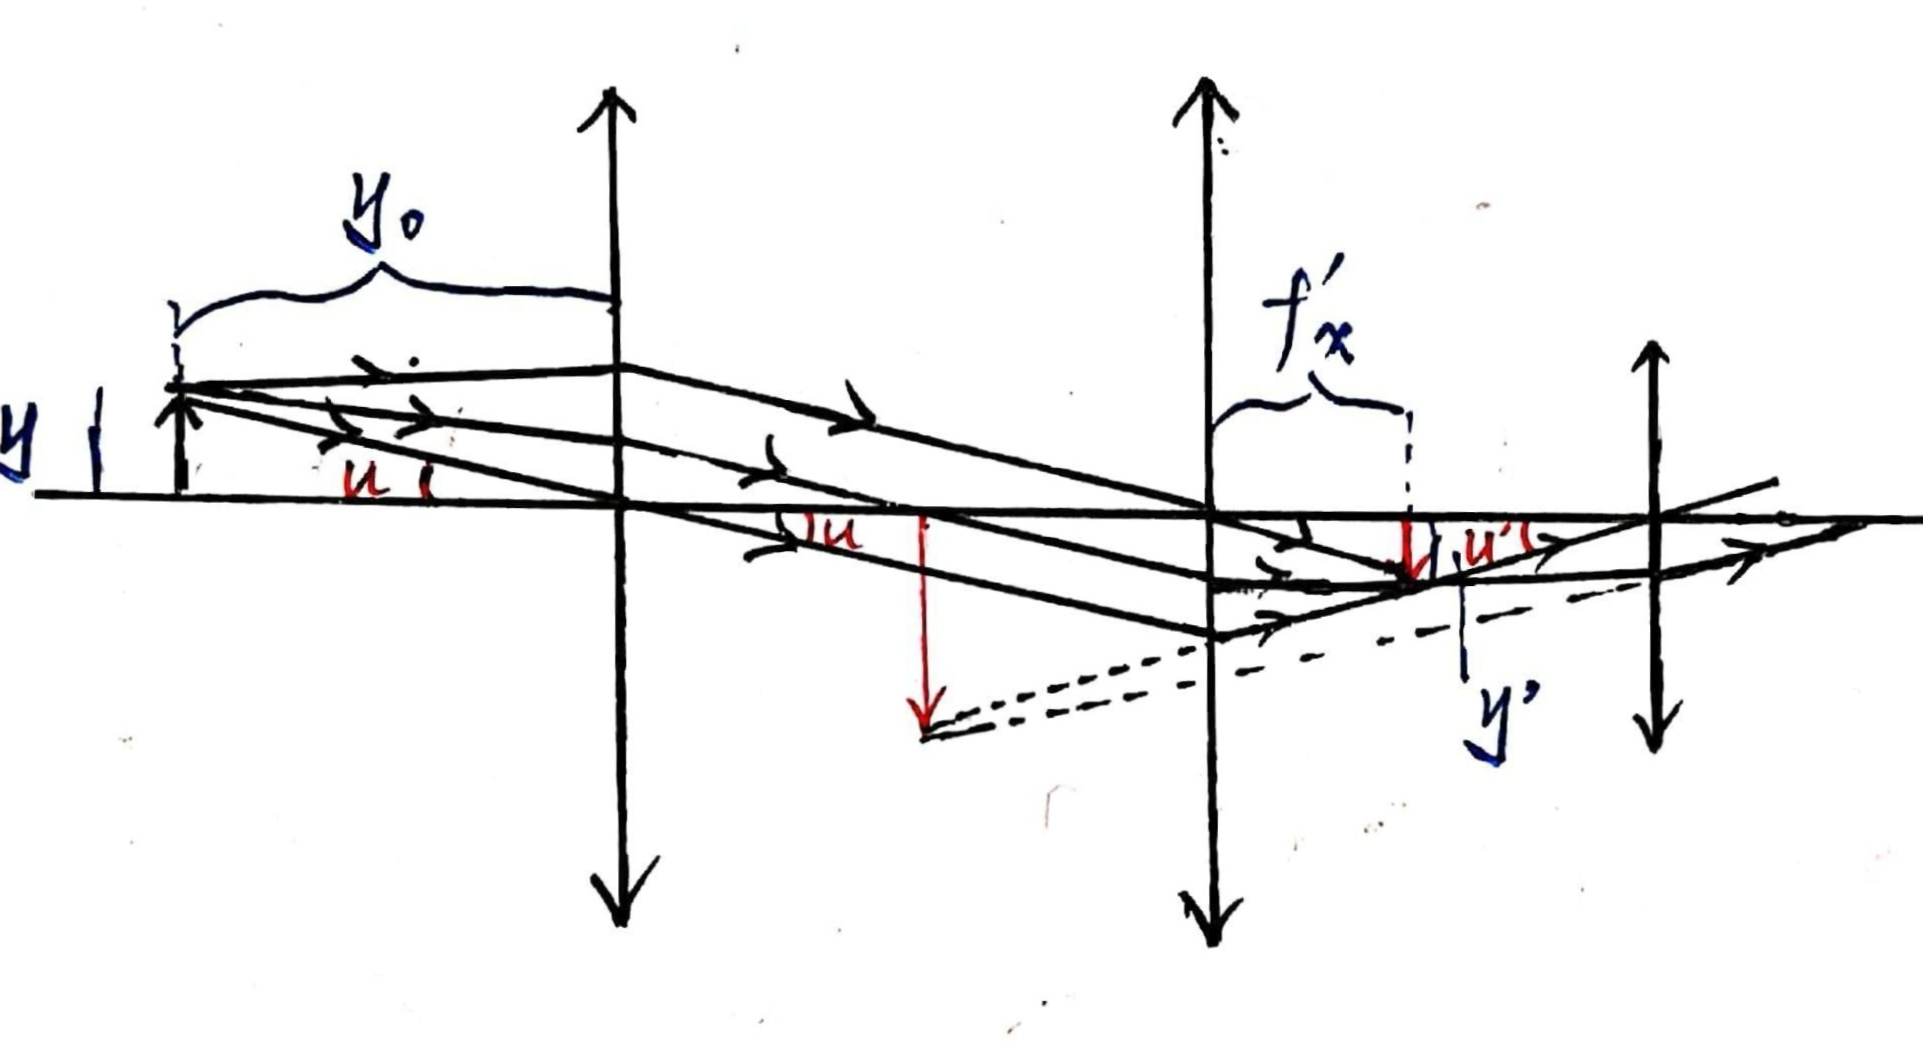
\includegraphics[scale=0.2]{1.jpg}\vspace{0em}
    \caption{焦距仪法测凸透镜焦距原理图}
    \end{center}
\end{figure}
可以看出,玻罗板上线对放置于平行光管物镜焦距处,射出平行光,待测透镜聚焦后,由测微目镜接收. 设平行光管物镜焦距为$f_0$,待测透镜焦距为$f’_x$,设光管出射平行光与主光轴夹角为$u$,待测透镜成的像对测微目镜光心张角为$u'$,考虑到测微目镜成虚像不改变张角$u'$,则有关系式:
\[\tan u=\frac{y}{f_0}\]
\[\tan u'=\frac{y'}{f'_x}\]
而由透过待测透镜光心的光线方向不改变有$u=u'$,联立各式得:
\begin{equation}
\label{jiaojuyifa}
f'_x=f_0\frac{y'}{y}
\end{equation}
在实验中,我们将平行光管中的一对线对作为成像的物.选定一对平行光管中的线对,线对间距和平行光管物镜焦距已知,则$y$与$f_0$已知,再通过测微目镜测量两个线对在目镜中像的位置(目镜读数值)$y_{1}'$、$y_{1}'$,线对间距$y'=\big{|}y_1'-y_2'\big{|}$即为像的大小. 最后通过(\ref{jiaojuyifa})式即可计算出凸透镜焦距.\par
具体实验中,首先需要将平行光管、凸透镜和测微目镜共轴调节,其次需要旋转调节目镜,看清叉丝,最后需要调整测微目镜位置,使上下左右移动眼睛观察目镜中的像时像基本不改变位置,如此则已经消除视差. 准备工作进行完毕后再转动测微目镜的鼓轮读出线对位置. 需要注意的是,由于鼓轮转动时存在空程差,因此每一次测量时均需从测量点外侧的一定距离开始单方向转动鼓轮直至另一侧测量点. 一次测量完毕后将鼓轮旋至测量起点再进行第二次测量.\par

\paragraph{测量数据如下:}\quad\par
\begin{center}{平行光管物镜焦距$f_0=54.8625cm$\quad线对间距$y=4mm$}\end{center}
\begin{table}[H]\begin{center}
    \caption{焦距仪法测凸透镜焦距测量数据表}
    \begin{tabular}{|c|c|c|c|c|c|c|c|c|}
        \hline
        组别&1&2&3&4&5&6&7&8\\
        \hline
        左线对读数$y_2'$/mm&0.510&0.592&0.555&0.562&0.572&0.568&0.575&0.568\\
        \hline
        右线对读数$y_1'$/mm&2.792&2.880&2.816&2.842&2.845&2.864&2.855&2.849\\
        \hline
    \end{tabular}
\end{center}\end{table}

\paragraph{数据处理如下:}\quad\par
\quad\quad第一组\quad线对像间距$y'_1=\big{|}y'_{11}-y'_{21}\big{|}=\big{|}2.792mm-0.510mm\big{|}=2.282mm$\par\quad\quad\quad\quad\quad\quad透镜焦距$\displaystyle{f'_{x1}=f_0\frac{y'_1}{y}=54.8625cm\times \frac{2.282mm}{4mm}=31.30cm}$\par\vspace{1em}
\quad\quad第二组\quad线对像间距$y'_2=\big{|}y'_{12}-y'_{22}\big{|}=\big{|}2.880mm-0.592mm\big{|}=2.288mm$\par\quad\quad\quad\quad\quad\quad透镜焦距$\displaystyle{f'_{x2}=f_0\frac{y'_2}{y}=54.8625cm\times \frac{2.288mm}{4mm}=31.38cm}$\par\vspace{1em}
\quad\quad第三组\quad线对像间距$y'_3=\big{|}y'_{13}-y'_{23}\big{|}=\big{|}2.816mm-0.555mm\big{|}=2.261mm$\par\quad\quad\quad\quad\quad\quad透镜焦距$\displaystyle{f'_{x3}=f_0\frac{y'_3}{y}=54.8625cm\times \frac{2.261mm}{4mm}=31.01cm}$\par\vspace{1em}
\quad\quad第四组\quad线对像间距$y'_4=\big{|}y'_{14}-y'_{24}\big{|}=\big{|}2.842mm-0.562mm\big{|}=2.280mm$\par\quad\quad\quad\quad\quad\quad透镜焦距$\displaystyle{f'_{x4}=f_0\frac{y'_4}{y}=54.8625cm\times \frac{2.280mm}{4mm}=31.27cm}$\par\vspace{1em}
\quad\quad第五组\quad线对像间距$y'_5=\big{|}y'_{15}-y'_{25}\big{|}=\big{|}2.845mm-0.572mm\big{|}=2.273mm$\par\quad\quad\quad\quad\quad\quad透镜焦距$\displaystyle{f'_{x5}=f_0\frac{y'_5}{y}=54.8625cm\times \frac{2.273mm}{4mm}=31.18cm}$\par\vspace{1em}
\quad\quad第六组\quad线对像间距$y'_6=\big{|}y'_{16}-y'_{26}\big{|}=\big{|}2.864mm-0.568mm\big{|}=2.296mm$\par\quad\quad\quad\quad\quad\quad透镜焦距$\displaystyle{f'_{x6}=f_0\frac{y'_6}{y}=54.8625cm\times \frac{2.296mm}{4mm}=31.49cm}$\par\vspace{1em}
\quad\quad第七组\quad线对像间距$y'_7=\big{|}y'_{17}-y'_{27}\big{|}=\big{|}2.855mm-0.575mm\big{|}=2.280mm$\par\quad\quad\quad\quad\quad\quad透镜焦距$\displaystyle{f'_{x7}=f_0\frac{y'_7}{y}=54.8625cm\times \frac{2.280mm}{4mm}=31.27cm}$\par\vspace{1em}
\quad\quad第八组\quad线对像间距$y'_8=\big{|}y'_{18}-y'_{28}\big{|}=\big{|}2.849mm-0.568mm\big{|}=2.281mm$\par\quad\quad\quad\quad\quad\quad透镜焦距$\displaystyle{f'_{x8}=f_0\frac{y'_8}{y}=54.8625cm\times \frac{2.281mm}{4mm}=31.29cm}$\par\vspace{1em}
则透镜平均值为$\displaystyle{\overline{f'_x}=\frac{\sum_{i=1}^{8}f'_{xi}}{8}=\frac{31.30+31.38+31.01+31.27+31.18+31.49+31.27+31.29}{8}cm=31.27cm}$.\\
估算不确定度:\par
i)计算$f'_x$B类不确定度\par 
我们对第1组数据计算B类不确定度以代替$f'_x$B类不确定度$U_{f'_{Bx}}$. \par由$\displaystyle{f'_x=f_0'\frac{y'}{y}=f_0'\frac{y_1'-y_2'}{y}}$得
\[\ln f'_x=\ln f_0'+ln(y_1'-y_2')-\ln y\]
那么$f'_x$的相对不确定度就可以写作:
\begin{table}[H]
\begin{center}

    \begin{tabular}{r c l}
$\displaystyle{\frac{U_{f'_{Bx}}}{f'_x}}$&=&
$\displaystyle{\sqrt{(\frac{\partial ln f'_x}{\partial f_0'})^2(U_{f_0'})^2+(\frac{\partial ln f'_x}{\partial y_1'})^2(U_{y_1'})^2+(\frac{\partial ln f'_x}{\partial y_2'})^2(U_{y_2'})^2+(\frac{\partial ln f'_x}{\partial y})^2(U_{y})^2}}$\\

\quad&=&$\displaystyle{\sqrt{(\frac{U_{f_0'}}{f_0'})^2+(\frac{U_{y_1'}}{y_1'-y_2'})^2+(\frac{U_{y_2'}}{y_1'-y_2'})^2+(\frac{U_{y}}{y})^2}}$

    \end{tabular}
\end{center}
\end{table}

%$f'_x$的相对不确定度为$\displaystyle{\frac{U_{f'_{Bx}}}{f'_x}=\sqrt{(\frac{U_{f'_0}}{f'_0})^2+(\frac{U_{y}}{y})^2+(\frac{U_{y'}}{y'})^2+}}$. 

%\footnote{需要注意的是,这里$y'=y'_1-y'_2$,而$y'_1$、$y'_2$都是一次项,因此计算$f'_x$B类不确定度时就有$\frac{U_{f'_{Bx}}}{f'_x}=\sqrt{(\frac{U_{f'_0}}{f'_0})^2+(\frac{U_{y}}{y})^2+(\frac{U_{y'_1}}{y'_1-y'_2})^2+(\frac{U_{y'_2}}{y'_1-y'_2})^2}\\=\sqrt{(\frac{U_{f'_0}}{f'_0})^2+(\frac{U_{y}}{y})^2+(\frac{U_{y'}}{y'})^2}$,这是此式的由来.}\par
 我们约定测量$y'_{1}$和$y'_{2}$的测微目镜仪器误差限为$\Delta_{INS}=0.005mm$,单次测量$U_{y'_{1}}=U_{y'_{2}}=\Delta_{INS}=0.005mm$. %因为$y'=y'_1-y'_2$,则$\displaystyle{U_{y'}=\sqrt{(U_{y'_{1}})^2+(U_{y'_{2}})^2}=\sqrt{0.005^2+0.005^2}=0.007mm}$, 因此$y'$的相对不确定度为\\$\displaystyle{\frac{U_{y'}}{y'}=\frac{0.007mm}{2.282mm}=0.3\%}$. 
 我们同时约定平行光管物镜焦距的相对不确定度为$\displaystyle{\frac{U_{f'_0}}{f'_0}=0.03\%}$,玻罗板线对间距的相对不确定度为$\displaystyle{\frac{U_{y}}{y}=0.02\%}$. 综合以上,有:
 %\[\frac{U_{f'_{Bx}}}{f'_x}=\sqrt{(\frac{U_{f'_0}}{f'_0})^2+(\frac{U_{y}}{y})^2+(\frac{U_{y'}}{y'})^2}=\sqrt{(0.03\%)^2+(0.02\%)^2+(0.3\%)^2}=0.3\%\]\par
 \begin{table}[H]
    \begin{center}
    
        \begin{tabular}{r c l}
    $\displaystyle{\frac{U_{f'_{Bx}}}{f'_x}}$&=&
    $\displaystyle{\sqrt{(\frac{U_{f_0'}}{f_0'})^2+(\frac{U_{y_1'}}{y_1'-y_2'})^2+(\frac{U_{y_2'}}{y_1'-y_2'})^2+(\frac{U_{y}}{y})^2}}$\\
    
    \quad&=&$\displaystyle{\sqrt{(0.03\%)^2+(\frac{0.005mm}{2.792mm-0.510mm})^2+(\frac{0.005mm}{2.792mm-0.510mm})^2+(0.02\%)^2}=0.3\%}$
    
        \end{tabular}
\end{center}
\end{table}

 %\[\frac{U_{f'_{Bx}}}{f'_x}=\sqrt{(\frac{U_{f_0'}}{f_0'})^2+(\frac{U_{y_1'}}{y_1'-y_2'})^2+(\frac{U_{y_2'}}{y_1'-y_2'})^2+(\frac{U_{y}}{y})^2}\]
 则$f'_x$的B类不确定度约为$U_{f'_{Bx}}=f'_x\times \frac{U_{f'_{Bx}}}{f'_x}=31.30cm\times0.03\%=0.09cm$\\\par
 ii)计算$f'_x$A类不确定度\par 
由贝塞耳公式,透镜焦距标准偏差为
\[s_{f'_x}=\sqrt{\frac{\sum_{i=1}^{n}(f'_{xi}-\overline{f'_x})^2}{n-1}}\]
{\quad\small{$=\sqrt{\frac{(31.30-31.27)^2+(31.38-31.27)^2+(31.01-31.27)^2+(31.27-31.27)^2+(31.18-31.27)^2+(31.49-31.27)^2+(31.27-31.27)^2+(31.29-31.27)^2}{8-1}}cm=0.14cm$}}\par\vspace{0.5em}
利用Excel程序的tinv函数计算$p = 0.95$时的$t$因子$t_{0.95,6}=2.4469$,则$f'_x$的A类不确定度为\[U_{f'_{Ax}}=t_{p,v}\frac{s_{f'_x}}{\sqrt{n}}=2.4469\times\frac{0.14cm}{\sqrt{8}}=0.12cm\]\par
iii)$f'_x$不确定度的合成及结果表达\par
将$f'_x$的A、B类不确定度合成得到$\displaystyle{U_{f'_{x}}=\sqrt{(U_{f'_{Ax}})^2+(U_{f'_{Bx}})^2}=\sqrt{0.09^2+0.12^2}cm=0.15cm}$. 综上,可将长焦透镜焦距的实验测量值表示为$f'_x=(31.27\pm0.12)cm$.

\subsection*{ C) 用读数显微镜测透镜主面间距}
\subsubsection*{C.1 主面间距测量}
\paragraph{实验原理及操作如下:}\quad\par
考虑到通过读数显微镜成清晰像时物距是一定的,则测量物的间距,可以直接等效为读数显微镜成清晰像时的位置差. 在此种情境中,平行光管透过透镜成的像与透镜后框距离之差$d_{BH'}$即可等效为读数显微镜看到玻罗板透过透镜成的像时的坐标$z_{F'}$和看到透镜后框时的坐标$z_{B}$之差,因此有$d_{BH'}=\big{|}z_{F'}-z_{B}\big{|}$. 将透镜旋转180°,同理有$d_{AH}=\big{|}z_{F}-z_{A}\big{|}$. 测出透镜外框厚度$d$,并采用B.2焦距计算值作为$f$的近似值,从而有:
\begin{equation}
    \label{e_b}
    e_b=\big{|}z_H-z_{H'}\big{|}=d_{AH}+d_{BH'}+d-2f
\end{equation}
具体实验中,我们需先调整平行光管、凸透镜和读数显微镜共轴平行,调整完成后瞄准玻罗板线的像使其与叉丝消视差,读出显微镜坐标$z_{F'}$,然后调整显微镜高度,目测使其对准透镜外框,向前推动显微镜,待像清晰后读出显微镜坐标$z_{B}$. 之后将透镜翻转180°,进行类似操作得到$z_{F}$和$z_{A}$. 操作完成后,还需用数显卡尺读出透镜外框厚度$d$.

\paragraph{测量数据如下:}\quad\par
\begin{center}
透镜外框厚度\quad$d=14.23mm=1.423cm$\\
B.2计算出的透镜焦距\quad$f=15.61cm$
\end{center}
\begin{table}[H]
\begin{center}
    \caption{主面间距测量原始数据表}
\resizebox{\textwidth}{!}{
    \begin{tabular}{|c|c|c|c|}
        \hline
        观察像方显微镜坐标$z_{F'}/cm$&观察像方显微镜坐标$z_{B}/cm$&观察物方显微镜坐标$z_{F}/cm$&观察物方显微镜坐标$z_{A}/cm$\\
        \hline
        65.15&80.52&65.46&80.48\\
        \hline
    \end{tabular}
}
\end{center}
\end{table}
由此得到
\[d_{BH'}=\big{|}z_{F'}-z_{B}\big{|}=\big{|}65.15cm-80.52cm\big{|}=15.37cm\]
\[d_{AH}=\big{|}z_{F}-z_{A}\big{|}=\big{|}65.46cm-80.48cm\big{|}=15.02cm\]
由(\ref{e_b})式得:
\[e_b=d_{AH}+d_{BH'}+d-2f=15.02cm+15.37cm+1.423cm-2\times15.61cm=0.59cm\]
即计算出的主面间距为$e_b=0.59cm$.

\subsubsection*{C.2 用主面间距修正共轭法测焦距中的系统误差}
\paragraph{实验原理如下:}\quad\par
从原理上讲,若透镜主面间存在间距,则B.2共轭法测凸透镜焦距过程中$a'=l-l'=\big{|}(z_{L1}-e_b/2)-(z_{L2}-e_b/2)\big{|}=\big{|}z_{L1}-z_{L2}\big{|}=a$依然不变,而$b'=l+l'=(z_{L1}-e_b/2)+(z_{L2}-e_b/2)=\big{|}z_{O}-z_{I}\big{|}-e_b=b-e_b$发生改变. 对B.2的数据计算进行修正可以得到:
\[b'=b-e_b=90.00cm-0.59cm=89.41cm\]
\[f'=\frac{b'^2-a^2}{4b'}=\frac{89.41^2-49.79^2}{4\times89.41}cm=15.41cm\]
可以看到,此结果与B.2计算出的结果$f=15.61cm$有一定差距,但总体上偏差不大.

\subsection*{ D) 用焦距仪测凹透镜焦距的附加透镜法}
\subsubsection*{D.1 测量视放大率}

\paragraph{实验原理及操作如下:}\quad\par
\begin{figure}[H]
    \begin{center}
    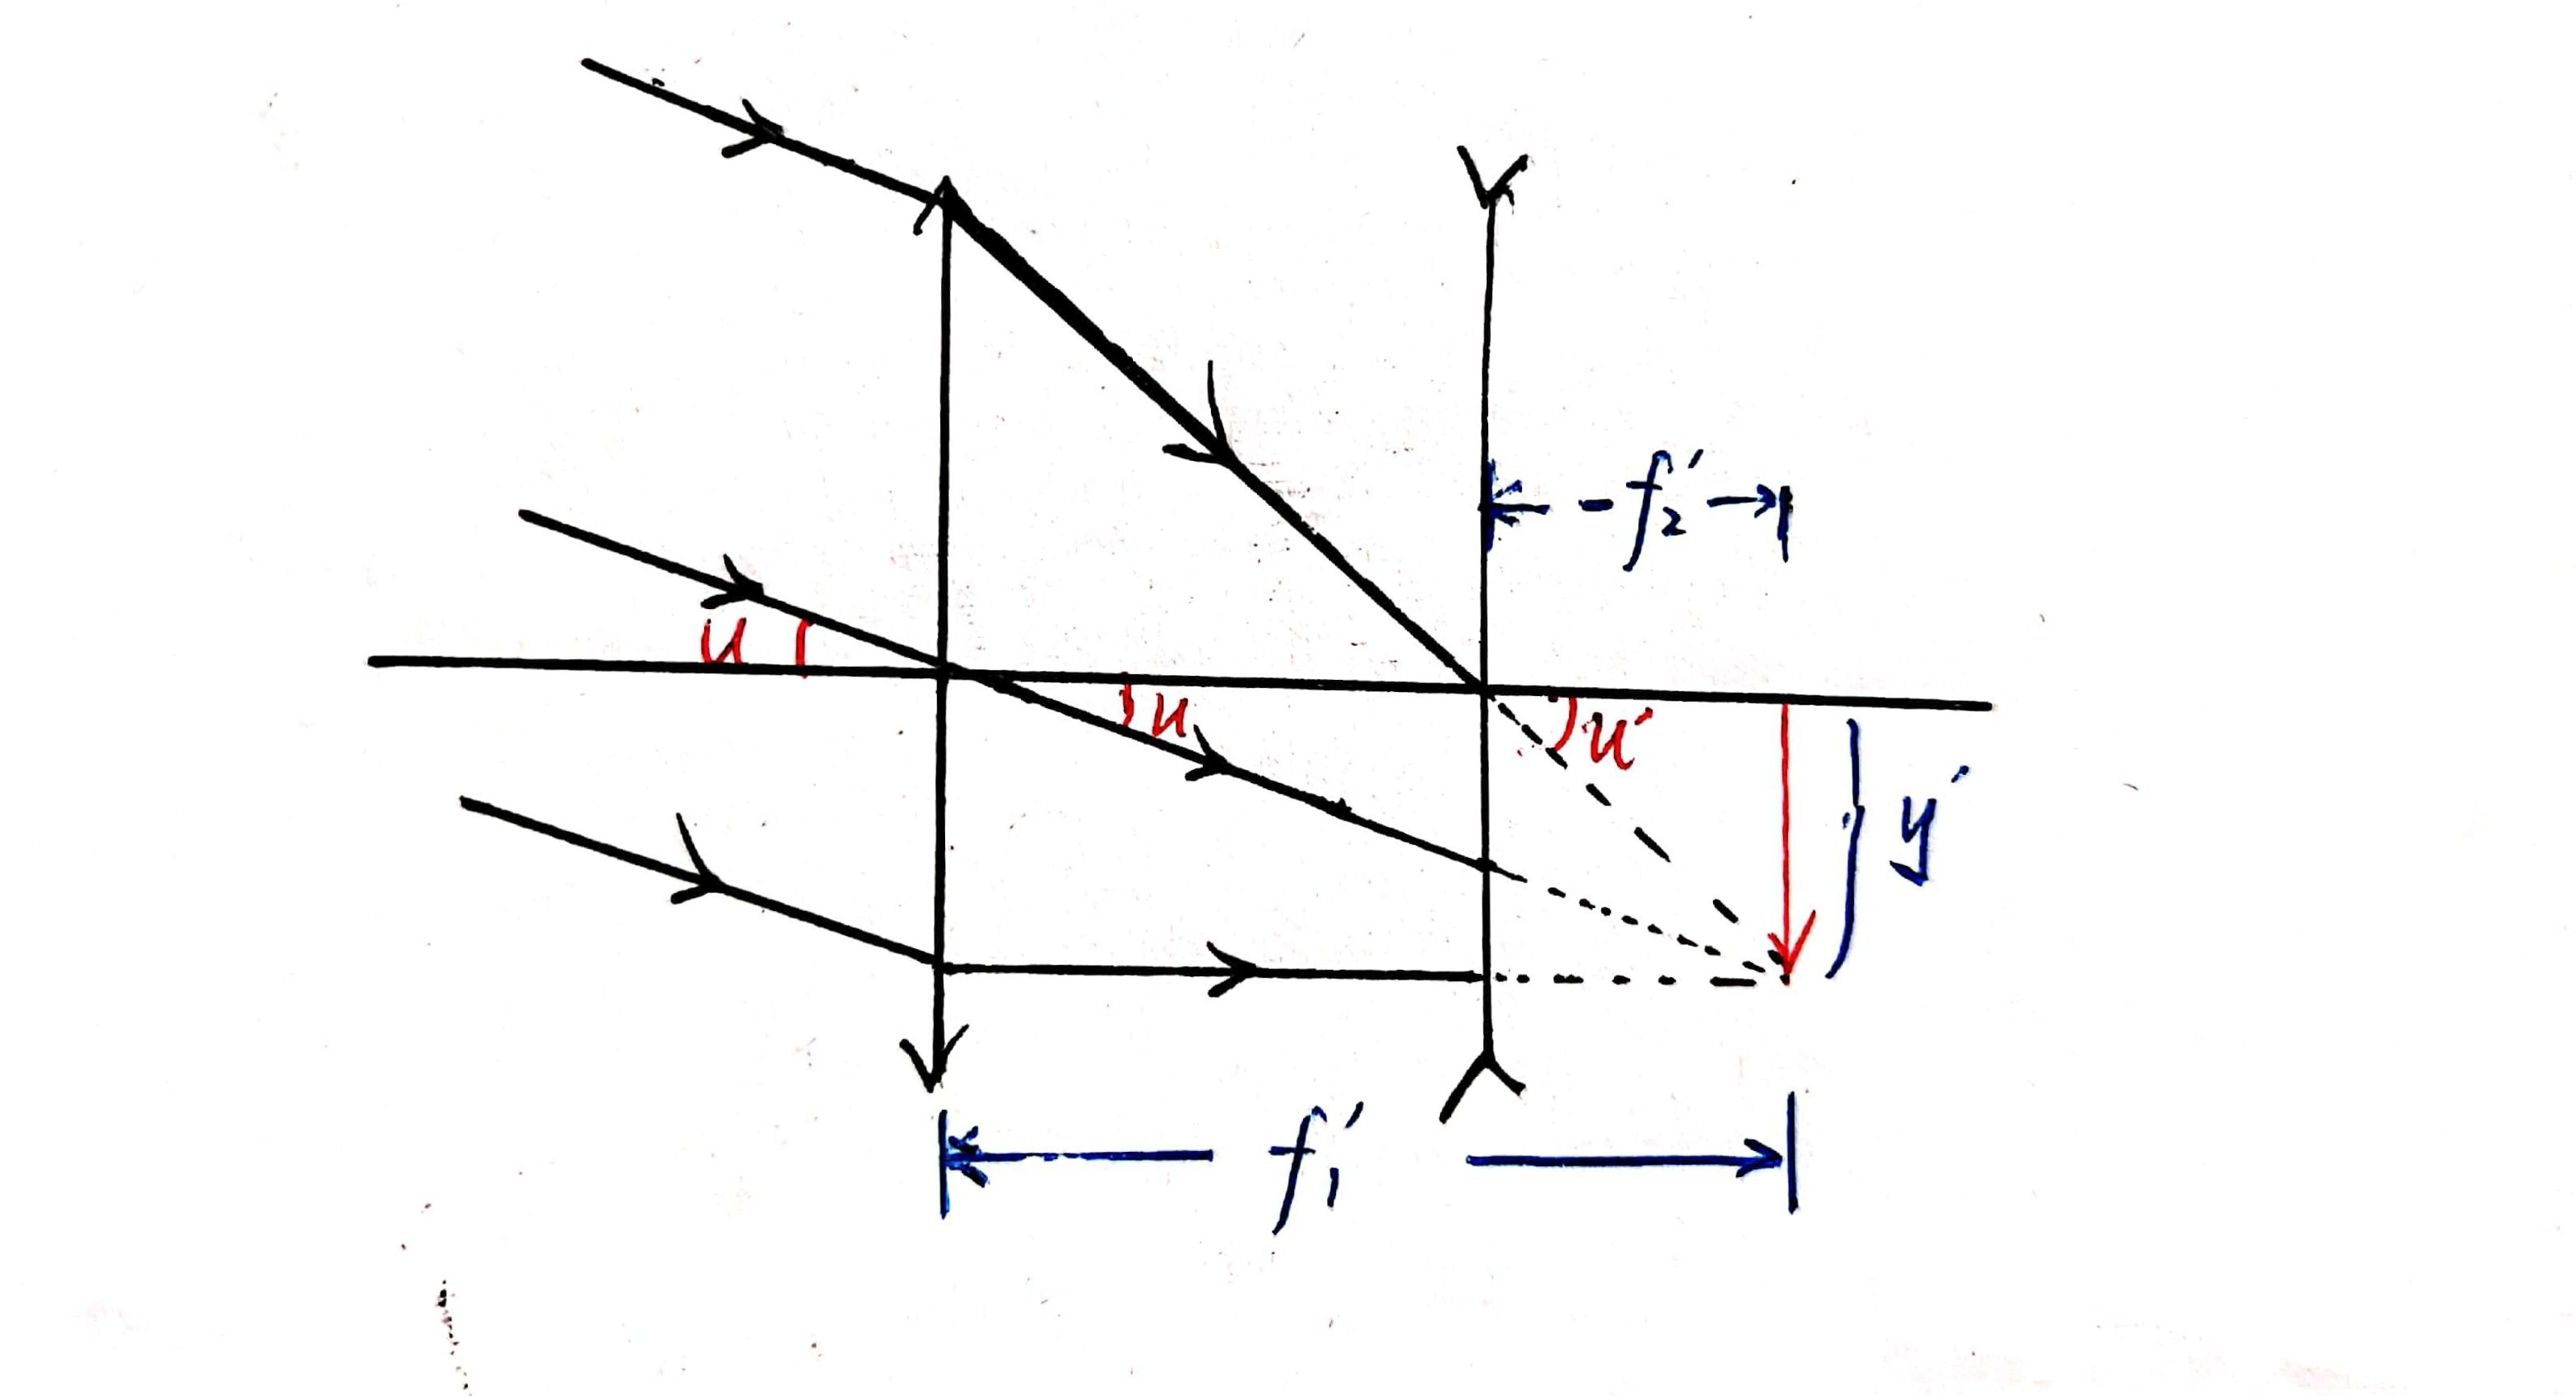
\includegraphics[scale=0.15]{2.jpg}\vspace{0em}
    \caption{用焦距仪测凹透镜焦距的附加透镜法原理图}
    \end{center}
\end{figure}
对于一个凹透镜焦点和凸透镜焦点重合的伽利略望远系统,由下图可知设凸透镜焦距$f'_1$,凹透镜焦距$f'_2$$(f'_1>f'_2)$,则有关系式
\[u_1\approx\tan u_1=\frac{y'}{f_1'}\]
\[u_2\approx\tan u_2=\frac{y'}{-f_2'}\]
则该望远系统角放大率为
\begin{equation}
    \Gamma=\frac{u_2}{u_1}=-\frac{f_1'}{f_2'}
\end{equation}
同样,我们也可以通过测量添加该望远系统前后的某一物成像的大小比衡量角放大率,具体来说,可以选定平行光管一对线对加某一透镜成像并用测微目镜测量像中线对间距$y_0$,再加望远系统测量像中线对间距$y''$,则有关系式
\begin{equation}
    \Gamma=\frac{y''}{y_0}
\end{equation}
则由以上两式,得:
\begin{equation}
    \big{|}f_2'\big{|}=\frac{f_1'}{\Gamma}={f_1'}\frac{y_0}{y''}
\end{equation}
具体到实验操作,我们先共轴调节,并用测微目镜观察平行光管射出的平行光通过复合透镜(未知透镜)成的像并测量其中一对线对间距$y_0$(左线坐标$y_{01}$,右线坐标$y_{02}$,则$y_0=y_{02}-y_{01}$),再依次加入长焦透镜(已知透镜)、凹透镜进行两次共轴调节,然后移动凹透镜位置直到能够看清线对的像,测量同一线对的间距$y''$(左线坐标$y''_{1}$,右线坐标$y''_{2}$,则$y''=y''_{2}-y''_{1}$),再通过(6)-(8)式完成计算.\par

\paragraph{测量数据如下:}\quad\par
选取间距为10mm的线对进行观测.
\begin{table}[H]\begin{center}
    \caption{附加透镜法测凹透镜焦距原始数据表}
\resizebox{\textwidth}{!}
{
    \begin{tabular}{|c|c|c|c|}
        \hline
        插入望远系统前读数1\quad$y_{01}/mm$&插入望远系统前读数2\quad$y_{02}/mm$&插入望远系统后读数1\quad$y''_{1}/mm$&插入望远系统后读数2\quad$y''_{2}/mm$\\
        \hline
        0.572&3.422&0.554&4.548\\
        \hline
    \end{tabular}
}
\end{center}\end{table}

\paragraph{数据处理如下:}\quad\par
\begin{center}
    插入望远系统前像中线对间距\quad$y_0=y_{02}-y_{01}=3.422mm-0.572mm=2.850mm$\\
    插后望远系统前像中线对间距\quad$y''=y''_{2}-y''_{1}=4.548mm-0.554mm=3.994mm$\\
    望远系统的视放大率\quad$\displaystyle{\Gamma=\frac{y''}{y_0}=\frac{3.994mm}{2.850mm}=1.401}$
\end{center}
\subsubsection*{D.2 计算凹透镜焦距}
B.3测量出的长焦透镜焦距为$f_1'=31.27cm$,代入(8)式得,
\begin{center}凸透镜焦距\quad$\displaystyle{\big{|}f_2'\big{|}=\frac{f_1'}{\Gamma}=\frac{31.27cm}{1.401}=22.32cm}$\end{center}


\subsection*{ E) 内调焦望远镜的物镜组研究}
\subsubsection*{E.1 自组内调焦望远镜的探究}

\paragraph{实验原理及操作如下:}\quad\par
根据理想透镜组成像的理论计算,设两个透镜焦距\footnote{考虑到实验条件下物方焦距与像方焦距相等,故不做严格区分;同时,认为透镜为薄透镜,因此物方像方主点与透镜光心重合.}分别为$f_1$、$f_2$,且光心间距为$d$,则对于组成的透镜组等效焦距(推导过程可见思考与讨论),有:
\begin{equation}
    \label{f_0}
    f_0=-\frac{f_1f_2}{d-f_1-f_2}
\end{equation}
由此,我们用一个凸透镜和一个凹透镜组成的透镜组等效为凸透镜作为简易内调焦望远镜的目镜,实验时在透镜组后加上测微目镜观察,则构成完整的望远系统. 验证时,我们可以通过两种办法测量透镜组中透镜间距$d$,对比两种方法的测量值是否吻合,从而达到验证的目的.\par
\textbf{第一种测量$d$的方法是:}采用B.3的焦距仪法测焦距,固定目镜和凸透镜,移动凹透镜位置直至目镜中能够看到玻罗板线对的清晰像. 用测微目镜测量玻罗板上某一线对经透镜组成像的像宽$y'$,而平行光管物镜焦距$f_{\text{光管}}$与线对原始宽度$y$已知,即可通过(\ref{jiaojuyifa})式得到透镜组等效焦距$\displaystyle{f_0'=f_{\text{光管}}\frac{y'}{y}}$,再由(\ref{f_0})式得到透镜间距
\begin{equation}
    d=\displaystyle{-\frac{f_1f_2}{f_0}+f_1+f_2}
\end{equation}
    其中凸透镜、凹透镜焦距$f_1$、$f_2$已经分别由B.3、D.2测得,从而便测量出$d$的值.\par
\textbf{第二种测量$d$的方法是:}在第一种方法中,移动凹透镜直至测微目镜中能够看到玻罗板线对的清晰像时,直接测量凸透镜和凹透镜的坐标$z_1$、$z_2$,即可计算得$d'=\big{|}z_1-z_2\big{|}$.\par
对比$d$、$d'$,若两者吻合较好,则验证了实验原理和操作的正确性.\par
在实验中,我们进行两次验证,第一次保持凸透镜在目镜前$30-35cm$处,第二次将凸透镜再远离$10cm$,两次验证使验证结果更为可信.
\paragraph{测量数据如下:}\quad\par
\begin{table}[H]\begin{center}
    平行光管物镜焦距$f_{\text{光管}}=54.8625cm$\quad线对间距$y=4mm$
    \caption{自组内调焦望远镜原始数据表}
    
\resizebox{\textwidth}{!}
{
    \begin{tabular}{|c|c|c|c|c|c|}
        \hline
        组别&目镜坐标$z_e/cm$&凸透镜坐标$z_1/cm$&凹透镜坐标$z_2/cm$&左线对像目镜读数$y_1'/mm$&右线对像目镜读数$y_2'/mm$\\
        \hline
        1&40.00&72.50&49.18&0.852&4.418\\
        \hline
        2&40.00&82.50&63.38&0.755&5.805\\
        \hline
    \end{tabular}
}
\end{center}\end{table}

\paragraph{数据分析如下:}\quad\par
\paragraph{对于第一组数据}\quad\par
由第一种测量方法
\begin{center}
    线对像间距$y'=\big{|}y_1'-y_2'\big{|}=4.418mm-0.852mm=3.566mm$\\透镜组等效焦距$\displaystyle{f_0'=f_{\text{光管}}\frac{y'}{y}=54.8625cm\times\frac{3.566}{4}=48.91cm}$\\则透镜间距$d=\displaystyle{-\frac{f_1f_2}{f_0}+f_1+f_2}=-\frac{31.27\times(-22.32)}{48.91}cm+31.27cm+(-22.32)cm=23.22cm$
\end{center}
由第二种测量方法
\begin{center}
    实际透镜间距$d'=\big{|}z_1-z_2\big{|}=\big{|}72.50cm-49.18cm\big{|}=23.32cm$
\end{center}
对比两种方法,可见吻合情况较好,实验原理和操作的正确性得到初步验证.

\paragraph{对于第二组数据}\quad\par
由第一种测量方法
\begin{center}
    线对像间距$y'=\big{|}y_1'-y_2'\big{|}=5.805mm-0.755mm=5.050mm$\\透镜组等效焦距$\displaystyle{f_0'=f_{\text{光管}}\frac{y'}{y}=54.8625cm\times\frac{5.050}{4}=69.26cm}$\\则透镜间距$d=\displaystyle{-\frac{f_1f_2}{f_0}+f_1+f_2}=-\frac{31.27\times(-22.32)}{69.26}cm+31.27cm+(-22.32)cm=19.03cm$
\end{center}
由第二种测量方法
\begin{center}
    实际透镜间距$d'=\big{|}z_1-z_2\big{|}=\big{|}82.50cm-63.38cm\big{|}=19.12cm$
\end{center}
对比两种方法,可见吻合情况较好,实验原理和操作的正确性得到初步验证.

\paragraph{结合一、二组数据}我们发现:i)第一组数据透镜间距$d$大于第二组. ii)测量得联合透镜组焦距第一组($f'_0=48.91cm$)也小于第二组($f'_0=69.26cm$). iii)像方主点与凹透镜光心距离等于目镜坐标$z_e$与凹透镜坐标之差$z_2$,第一组为$x_H=z_2-z_e=49.18cm-40.00cm=9.18cm$,第二组为$x_{H'}=z_2-z_e=63.38cm-40.00cm=23.38cm$,可见第一组$x_H$也小于第二组. \par
而理论计算的公式为:$f=-\frac{f_1f_2}{d-f_1-f_2}$、$x_{H'}=f_2\frac{d}{d-f_1-f_2}$可见$d$减小,$f$增大,$x_H$增大,这与以上数据均符合,从定性分析角度,实验原理和操作的正确性得到进一步验证.


\subsubsection*{E.2 曲线绘制}
\begin{figure}[H]
    \begin{center}
    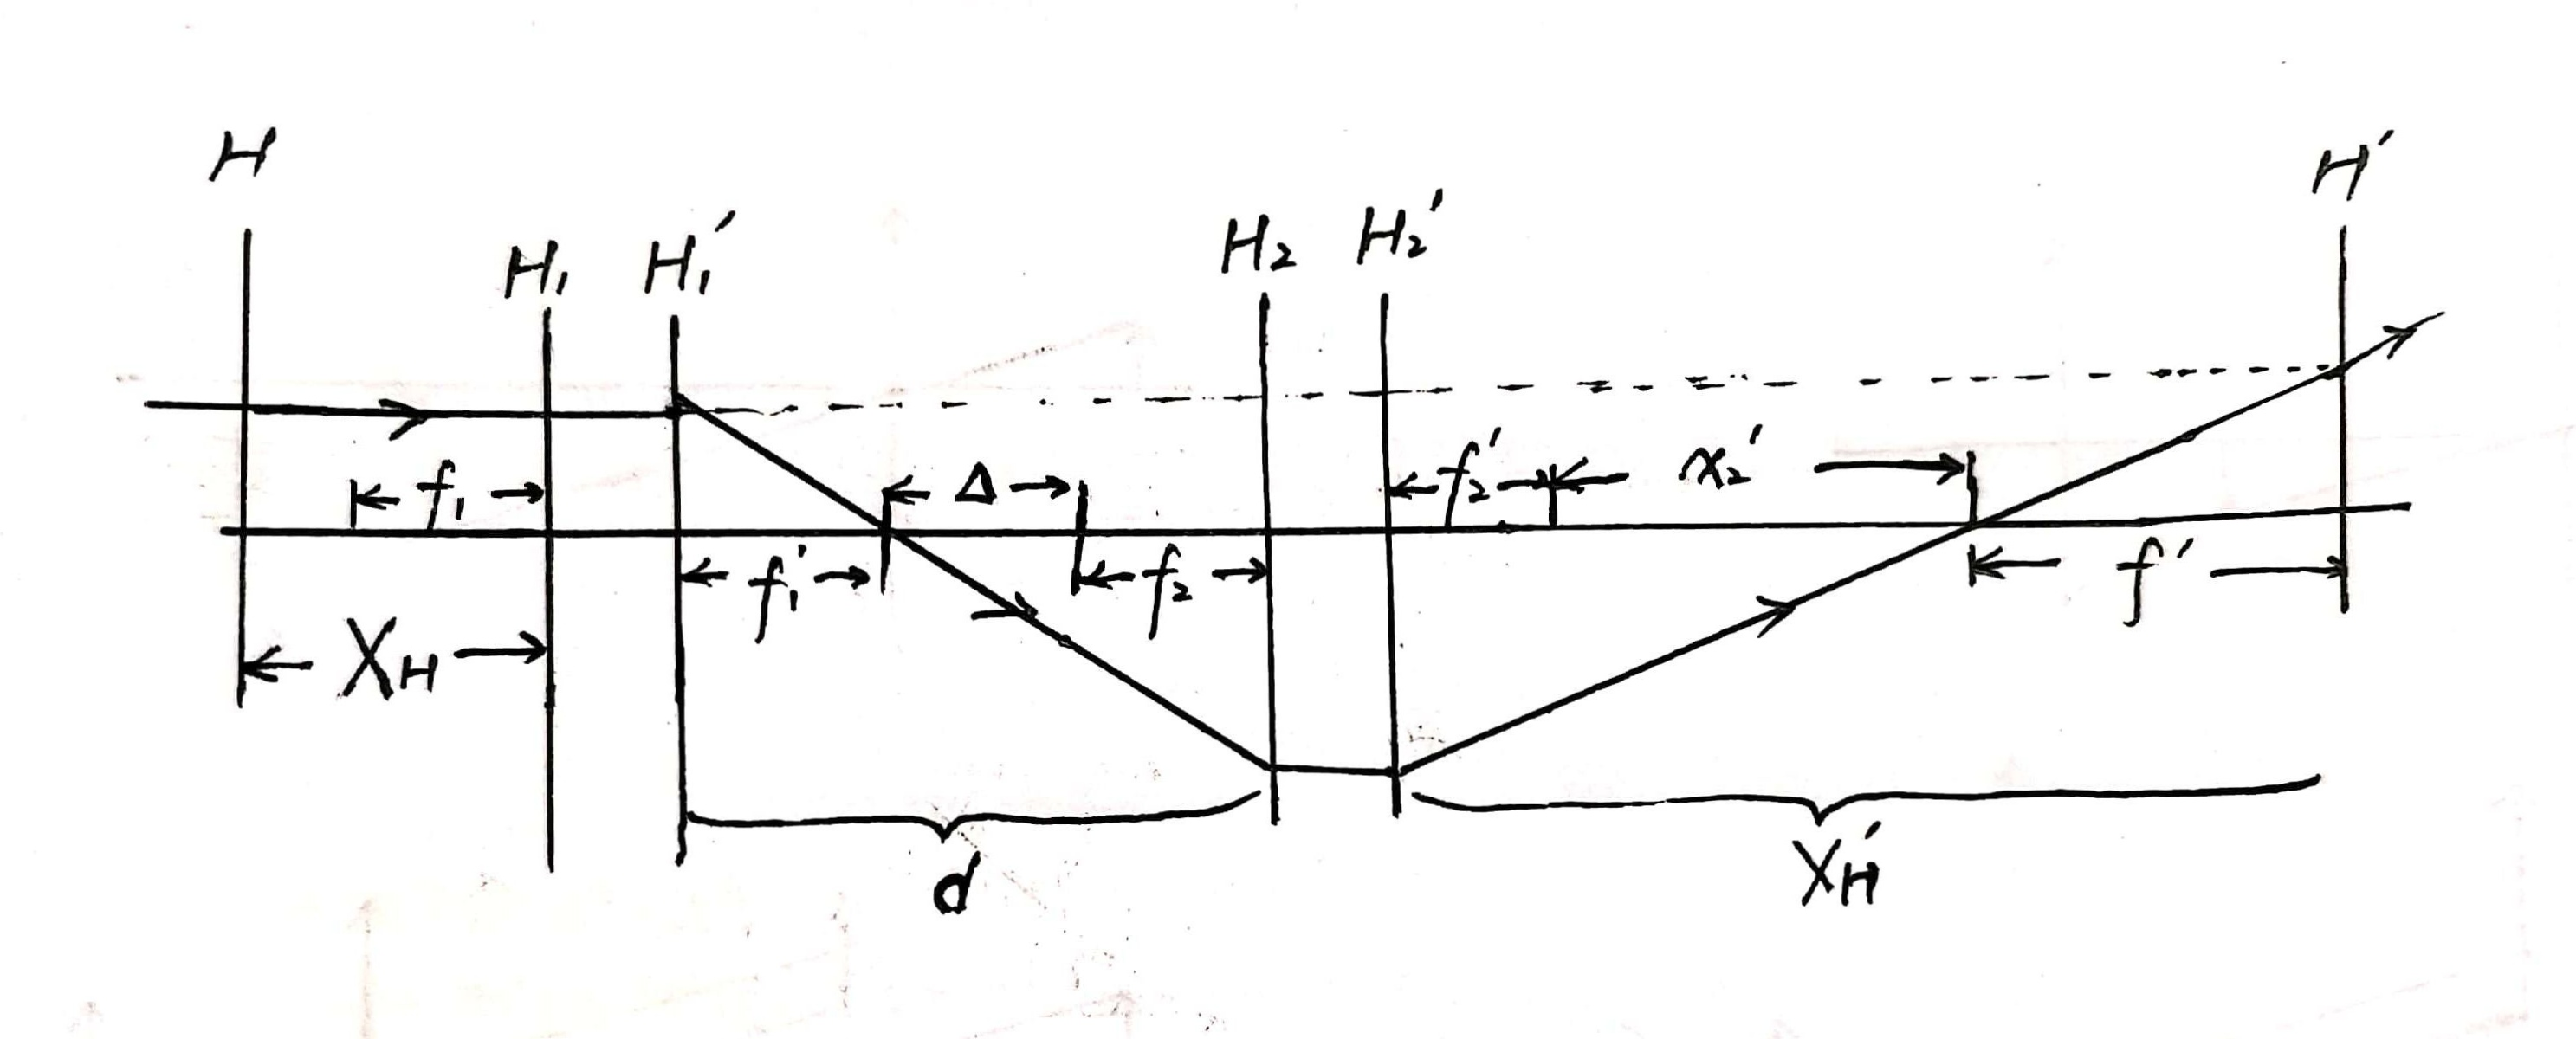
\includegraphics[scale=0.17]{3.jpg}\vspace{0em}
    \caption{理想透镜组成像原理图}
    \end{center}
\end{figure}
如图,由理想透镜组成像原理,我们可以推导出以下公式(推导过程见思考与讨论):
\begin{equation}
    f=-\frac{f_1f_2}{\Delta}=-\frac{f_1f_2}{d-f_1'-f_2}
\end{equation}
\begin{equation}
    f'=-\frac{f_1'f_2'}{\Delta}=-\frac{f_1'f_2'}{d-f_1'-f_2}
\end{equation}
\begin{equation}
    x_H=f_1\frac{d}{\Delta}=f_1\frac{d}{d-f_1'-f_2}
\end{equation}
\begin{equation}
    x_{H'}=f_2'\frac{d}{\Delta}=f_2'\frac{d}{d-f_1'-f_2}
\end{equation}
在实验中有$f_1=f_1'$,$f_2=f_2'$,并取凸透镜$f_1=0.3m=300mm$,凹透镜$f_2=-0.2m=-200mm$,绘图时要求以凸透镜位置作为零点,以物方至像方方向为正方向,结合给出的理想透镜组中各物理量示意图,我们只需分别绘制以下曲线\textbf{(下列各式中物理量的单位均为mm)}:
\[\text{透镜组焦距}\quad f_0=f=-\frac{f_1f_2}{d-f_1-f_2}=-\frac{300\times (-200)}{d-300-(-200)}=\frac{60000}{d-100}\]
\[\text{物方焦点坐标}\quad x_{f}=-(x_H+f)=\frac{f_1f_2-f_1d}{d-f_1-f_2}=\frac{300\times (-200)-300d}{d-300-(-200)}=-\frac{300d+60000}{d-100}\]
\[\text{像方焦点坐标}\quad x_{f'}=d+x_{H'}+f'=\frac{d^2-f_1d-f_1f_2}{d-f_1-f_2}=\frac{d^2-300d-300\times (-200)}{d-300-(-200)}=\frac{d^2-300d+60000}{d-100}\]
\[\text{物方主点坐标}\quad L_{1H}=-x_H=-\frac{f_1d}{d-f_1-f_2}=-\frac{300d}{d-300-(-200)}=-\frac{300d}{d-100}\]
\[\text{像方主点坐标}\quad L_{1H'}=d+x_{H'}=\frac{d^2-f_1d}{d-f_1-f_2}=\frac{d^2-300d}{d-300-(-200)}=\frac{d^2-300d}{d-100}\]
则绘制出的图像如下:
\begin{figure}[H]
    \begin{center}
    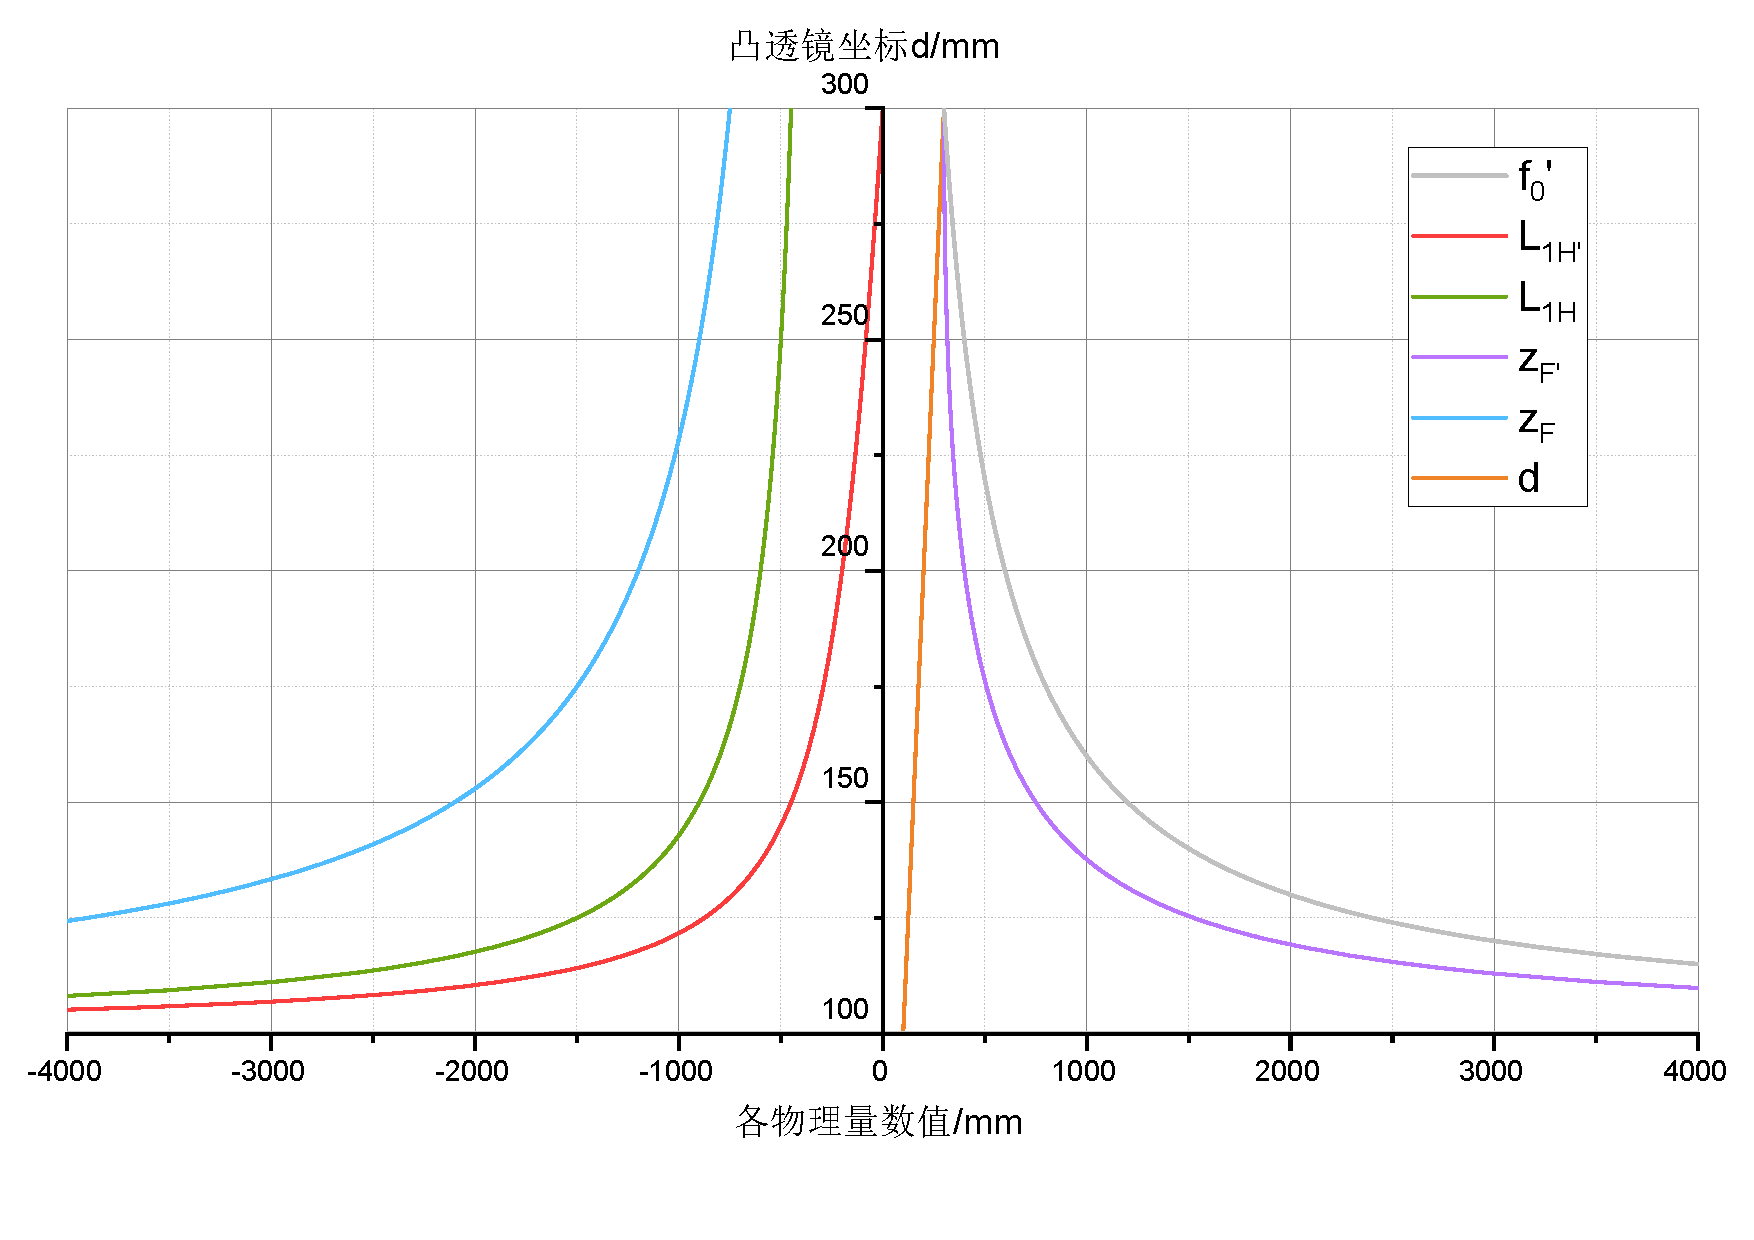
\includegraphics[scale=0.5]{graph.pdf}\vspace{-2.5em}
    \caption{凸凹透镜间距d和主点、焦点坐标等物理量的关系曲线}
    \end{center}
\end{figure}



\section{思考与讨论}
\paragraph{1.\quad 对E图像与数据的补充验证}\quad\par
在E中,我们选取E.1中任一组数据对E.2的图像含义进行进一步探究.\par
由B.3和D.2得到的凸透镜焦距$f_1=312.7mm$和$f_2=-223.2mm$,我们可以通过E.2中得到的各式绘制出各物理量理论曲线.\par
下面选取第一组数据进行验证. 第一组数据中目镜坐标$z_e=40.00cm$,凸透镜坐标$z_1=72.50cm$,凹透镜坐标$z_2=49.28cm$,计算出的$d=z_1-z_2=72.50cm-49.28cm=23.22cm=232.2mm$,为此我们在曲线中标出$d=232.2mm$的平行线,并描绘出它与各曲线的交点. 具体如下图所示:
\begin{center}\begin{figure}[H]
    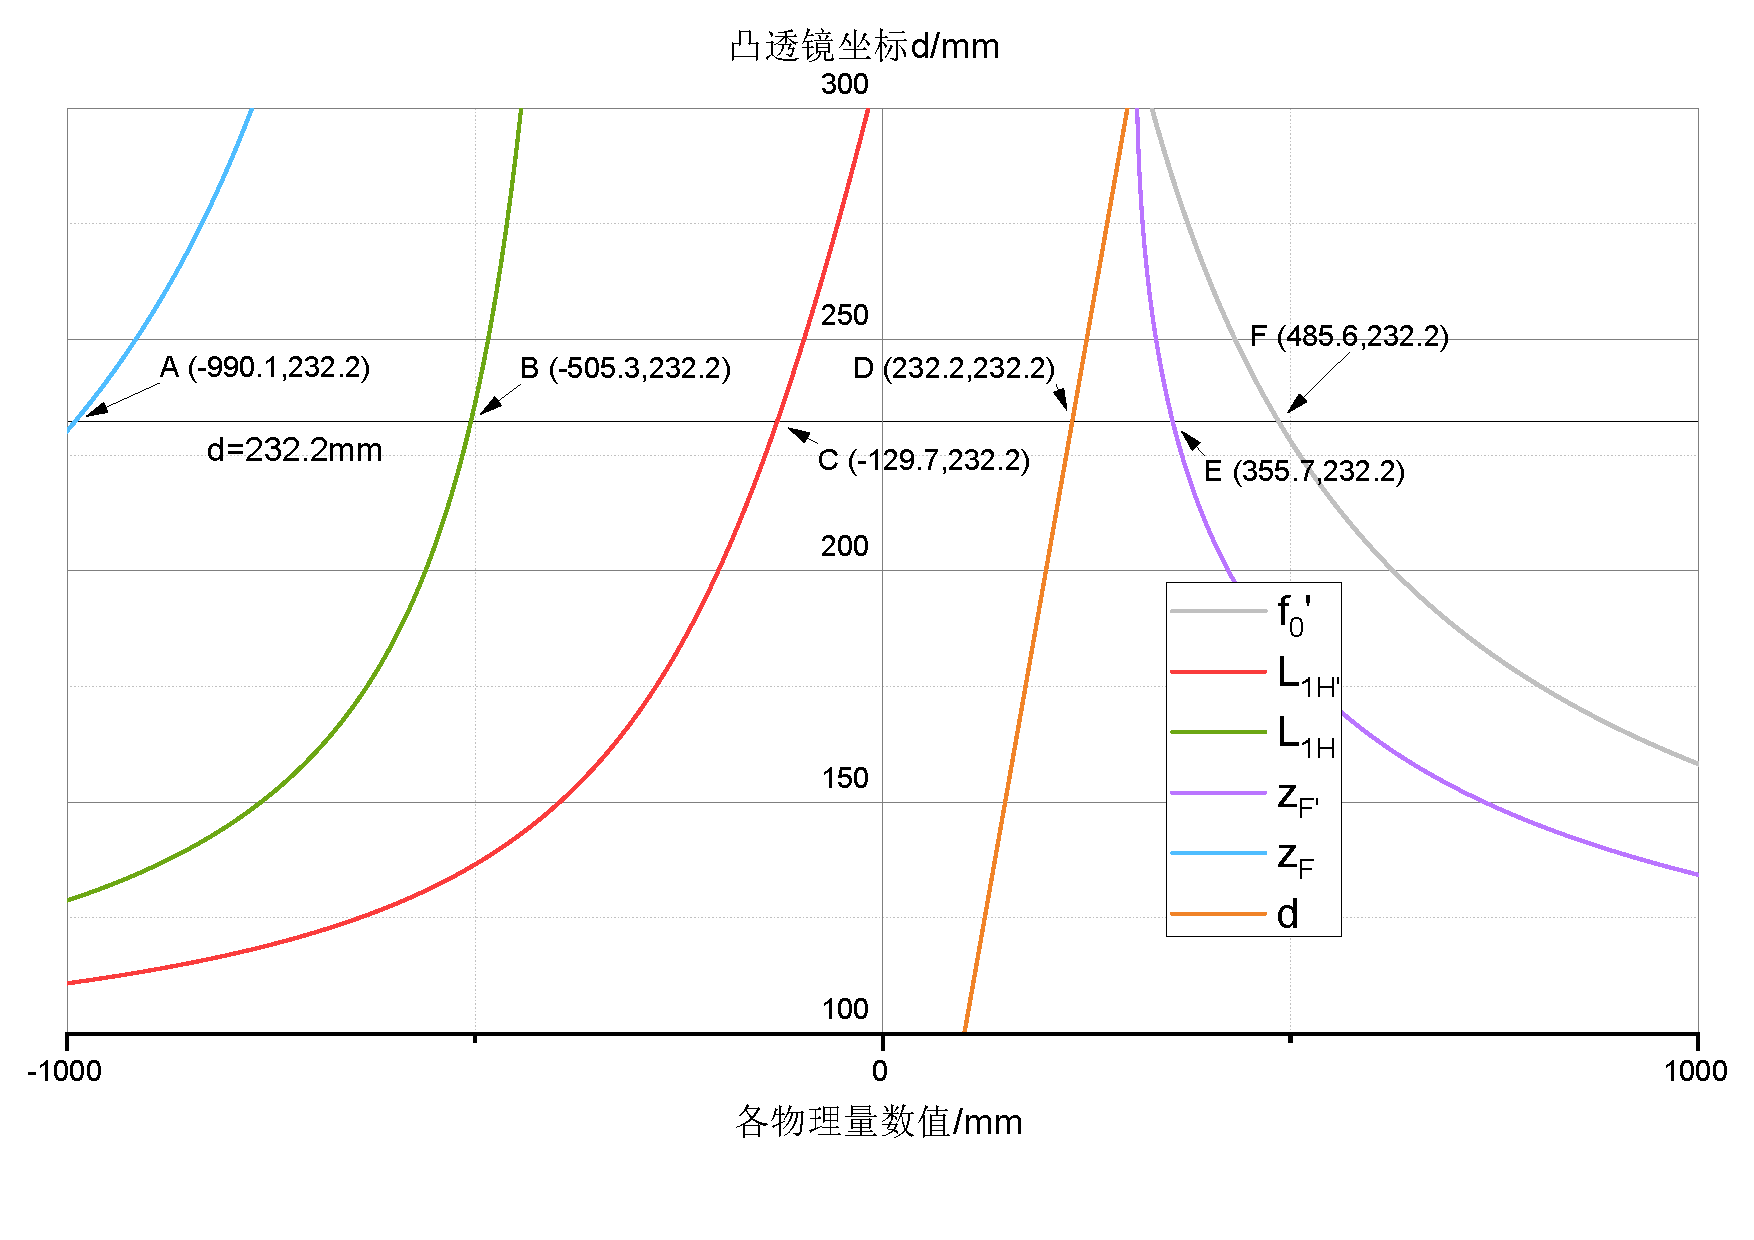
\includegraphics[scale=0.5]{graph1.pdf}
    \caption{E.1中第一组数据各物理量理论曲线}
    \vspace{-2.5em}
\end{figure}\end{center}
我们对第一组数据分析出的焦距进行验证.\par
\quad E.1计算出的透镜组焦距$f=489.1mm$,与图中F点横坐标$x_F=485.6mm$
比较接近. 同时,由假设,透镜均为薄透镜,因此像方主点与像方焦点坐标之差、物方主点与物方焦点坐标之差均表示透镜组焦距,在图上分别对应CE横坐标差和AB横坐标差. 读图得,CE横坐标差$x_E-x_C=355.7mm-(-129.7mm)=485.4mm$,AB横坐标差$x_B-x_A=(-505.3)mm-(-990.1mm)=484.8mm$,考虑到读图时存在一定误差,因此在误差限度内,以上关于焦距的计算值均符合较好,进一步验证了有关理想透镜组的相关原理和实验方法正确性.

\paragraph{2.\quad 关于本实验中采用测微目镜还是读数显微镜的讨论}\quad\par
分析测微目镜的构造,我们会发现它由一个分划板和一个目镜组成,成于分划板的像通过相当于放大镜的目镜被人眼看清,而读数显微镜则由物镜、目镜和夹在中间的分划板构成. 由结构可以分析,对于一般物体,无透镜则光屏上无像,因此无法用肉眼观察到,C部分实验需要观察透镜外框,中间无光学仪器,因此无法直接在测微目镜的光屏上成像,也就不能用测微目镜观察;而读数显微镜存在目镜,因此此部分实验只能采用读数显微镜. \par
事实上,本实验的其他部分也可以使用光学显微镜进行实验,但由于其物镜放大率不一定十分精确,无法保证总为1,且可以满足成像条件的景深是一个范围,会使微米级的测量出现不可避免的误差,因此当无需直接观察物体时,采用目镜也可以完成实验的部分,如B.3、D)、E)部分,尽量均用测微目镜.\par

\paragraph{3.\quad 空程差等实验注意事项}\quad\par
使用时需要格外注意,物理实验仪器中齿轮结构中存在间隙,因此反向时会存在较大的误差,称作空程差. 本实验中测量线对的像间距涉及转动测微目镜的鼓轮,因此测量时只能单方向转动. 测量前,将叉丝移至线对的范围之外,测量时再向里旋转与一侧的线对对齐读数,随后再单方向继续移动叉丝,直至与另一侧线对对齐,不可逆旋.

\paragraph{4.\quad 关于C)部分实验中主面间距测量的一些思考}\quad\par
i)\quad从B.2部分原理叙述可知,共轭法测非薄凸透镜会存在系统误差,主面不重合是其中的重要一点,为此我们用C)进行系差修正. C)部分实验逻辑为利用B.2测出的存在系差的焦距数据计算主面间距,再通过得到的主面间距修正B.2的测量结果. 但由于B.2存在系差,主面间距也必然存在系差,再进行修正也必然存在系差.\par
我认为一个理想的做法是设出主面$e$,并结合(\ref{gongefa})式(\ref{e_b})式得到:
\begin{equation}
    e=d_{AH}+d_{BH'}+d-2f=d_{AH}+d_{BH'}+d-2\frac{(b-e)^2-a^2}{4(b-e)}
\end{equation}
该方程中未知数仅有$e$,因此利用B.3和C.1得到的数据
$d_{BH'}=15.37cm$,$d_{AH}=15.02cm$,$d=1.423cm$,$a=49.79cm$,$b=90.00cm$,代入可解得:
\[e=1.70cm\]
此与C)部分得出的$e=0.59cm$存在较大差距,结合实验中许多同学测出负主面间距,我认为真实情况可能更接近于这种方法计算出的结果.\par\vspace{2em}
ii)\quad除此之外,还有一种消除误差的办法. 我们不妨设透镜光心与两个主点距离分别为$e_1$、$e_2$,一次成像中真实物距像距分别为$u_i$、$v_i$,并可以测量出透镜光心与物的距离$l_1$、与像的距离$l_2$,因此可以列出如下方程:
\begin{equation}
    \begin{cases}
        u_i+d_1=l_1\\
        v_i+d_2=l_2\\
        \frac{1}{v_i}+\frac{1}{u_i}=\frac{1}{f}
    \end{cases}
\end{equation}
一个方程式中可测量的量为$l_1$、$l_2$,未知量有$u_i$、$v_i$、$d_1$、$d_2$、$f$,但需要注意,一次成像实验可以多列一个方程组,多引入2个未知量($u, v$),但会带来三个等式,因此理论上只需要3组成像数据,联立3个方程组即可解出最终结果. 对于个人来说较为困难,但如果有大型计算工具,此种方法未必不可行.\par

\paragraph{5.\quad 理想光具组成像原理(11)-(14)式的证明}\quad\par
原理图和证明过程均见下:

\begin{figure}[H]
    \begin{center}
    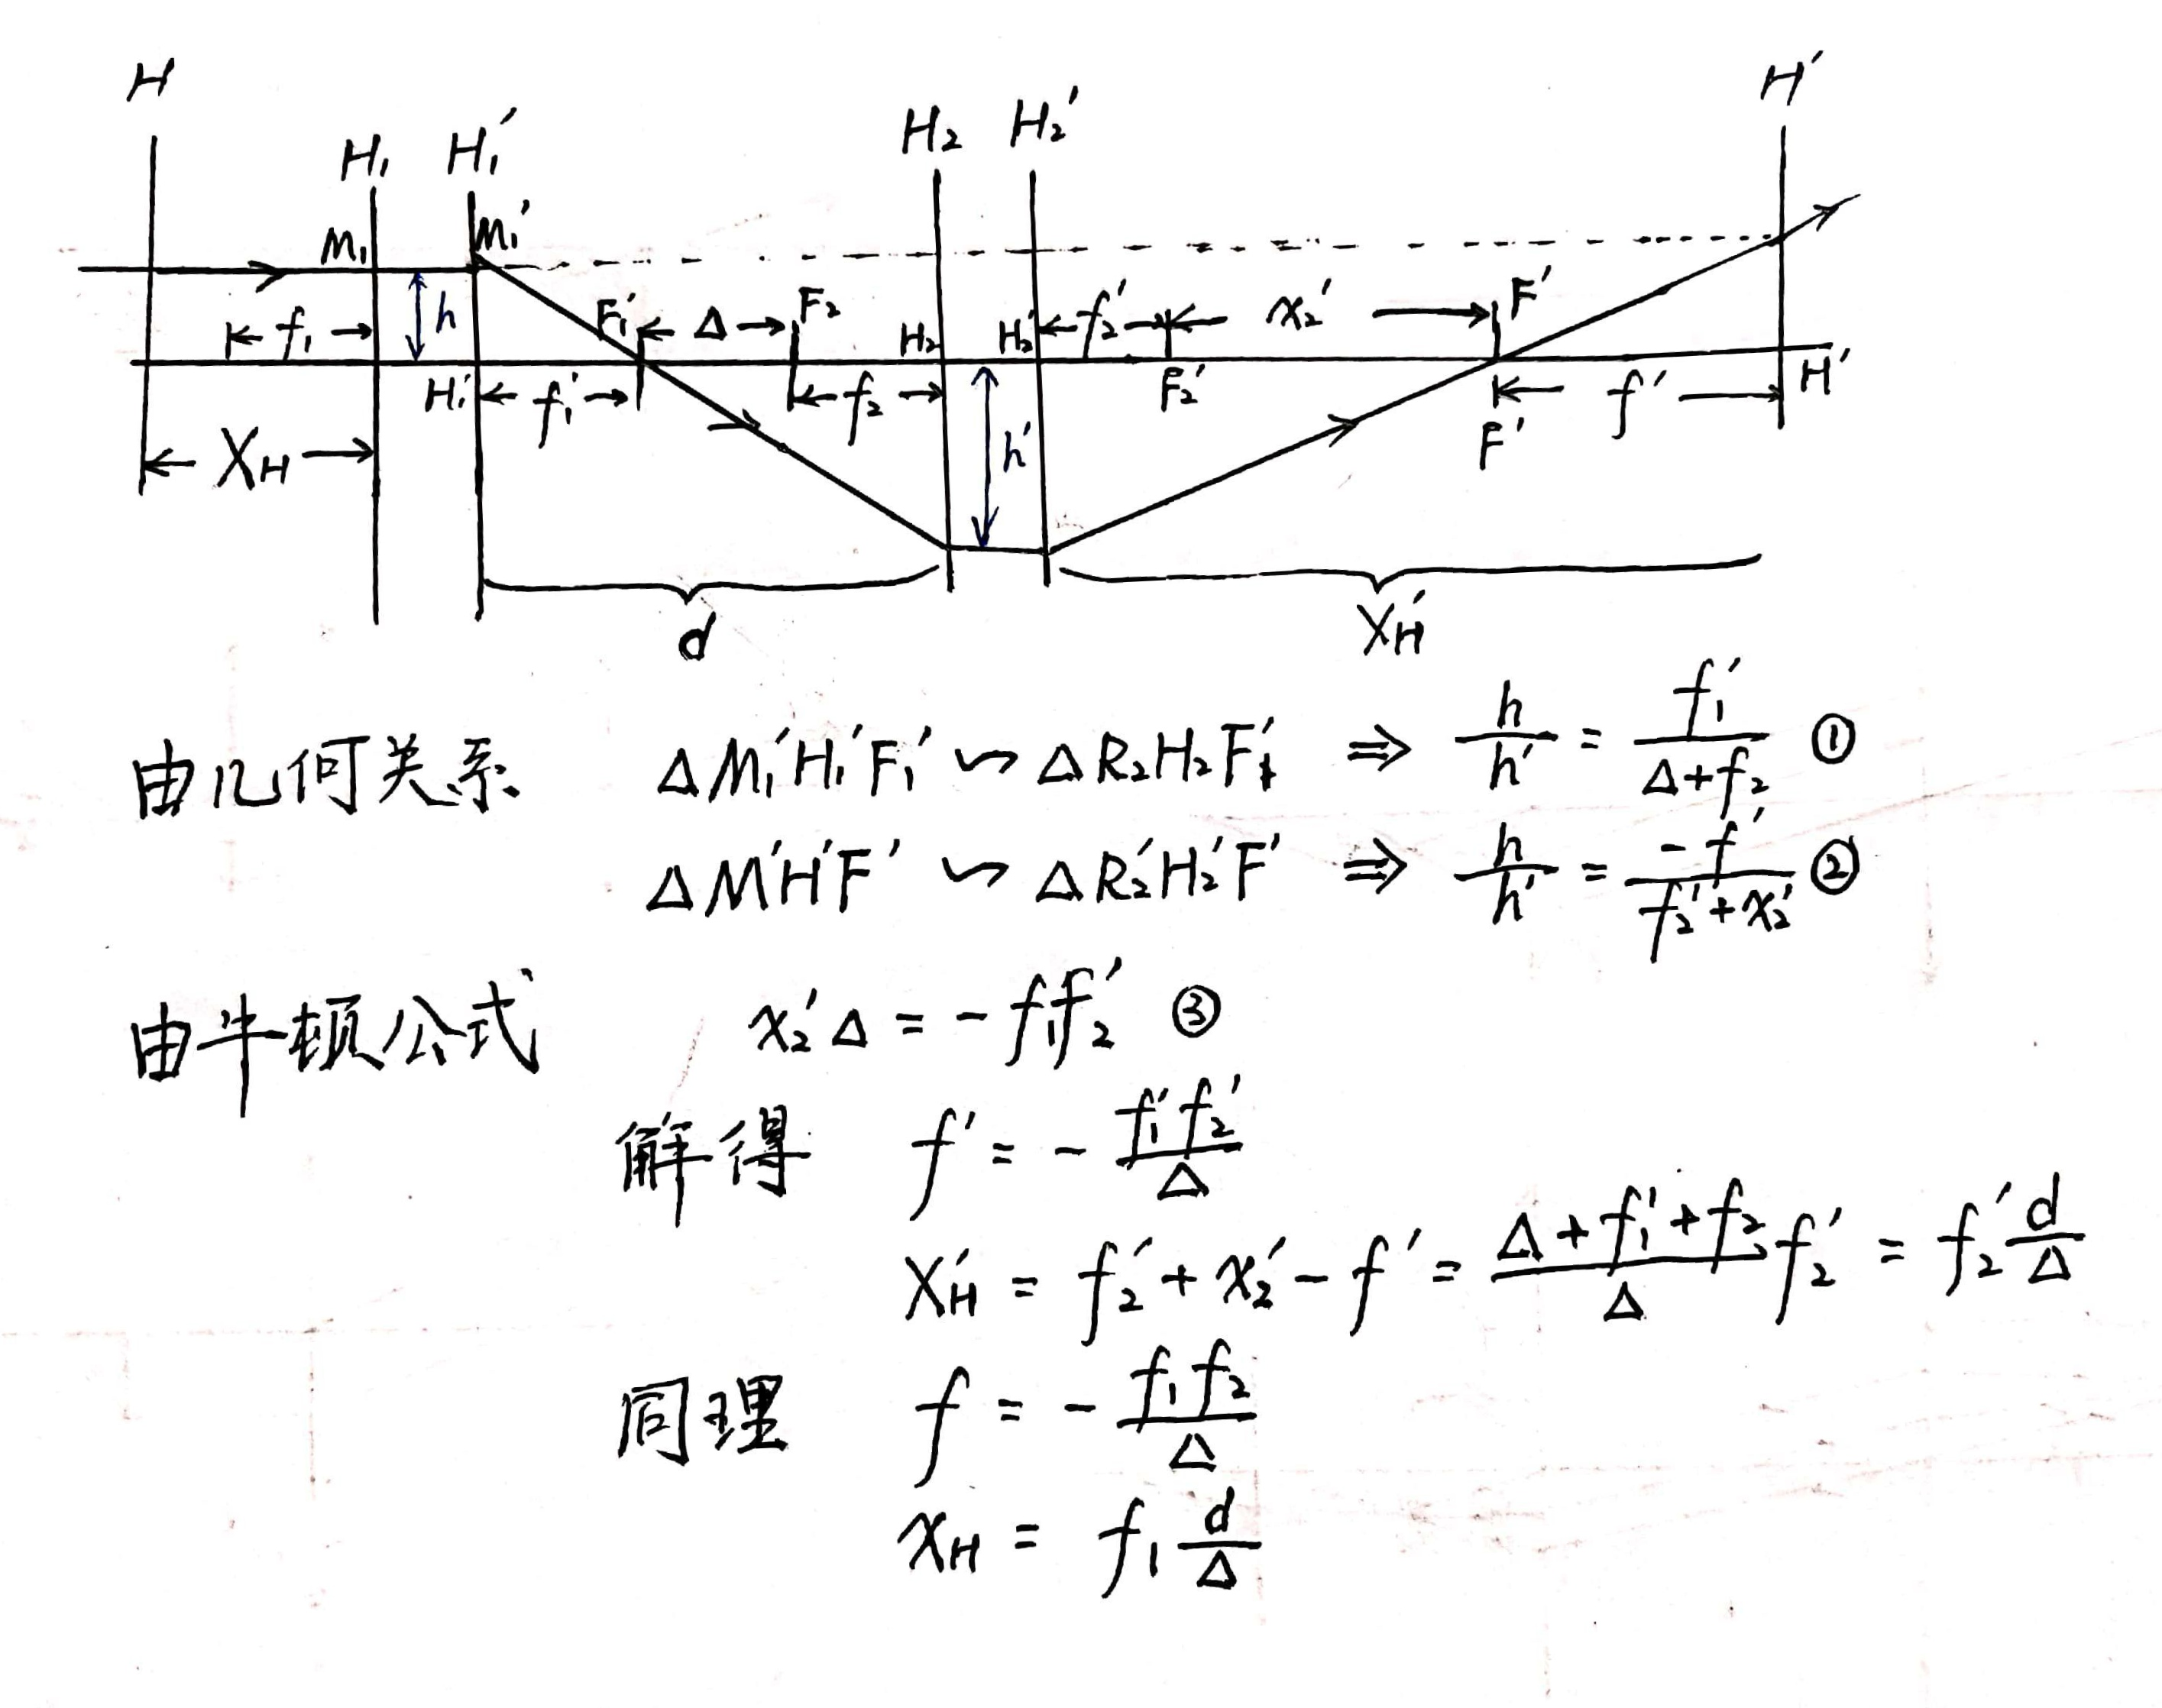
\includegraphics[scale=0.15]{4.jpg}\vspace{-2.5em}
    \caption{理想光具组成像原理证明过程}
    \end{center}
\end{figure}


\paragraph{6.\quad B.3中B类不确定度的另一种解法}\quad\par

我们在B.3原理部分已经推导出
$\displaystyle{f'_x=f_0'\frac{y'}{y}}$,那么用$\displaystyle{\frac{U_{f'_{Bx}}}{f'_x}=\sqrt{(\frac{U_{f'_0}}{f'_0})^2+(\frac{U_{y}}{y})^2+(\frac{U_{y'}}{y'})^2}}$也可以算出正确的不确定度. 即我们先计算中间变量$y$的不确定度,再基于此计算最终的不确定度,这种计算方法在此题中也是正确的. 证明如下:\par
我们已经利用相对不确定度的计算公式推导出$\displaystyle{\frac{U_{f'_{Bx}}}{f'_x}=\sqrt{(\frac{U_{f_0'}}{f_0'})^2+(\frac{U_{y_1'}}{y_1'-y_2'})^2+(\frac{U_{y_2'}}{y_1'-y_2'})^2+(\frac{U_{y}}{y})^2}}$,
这里$y'=y'_1-y'_2$,而$y'_1$、$y'_2$都是一次项,单次测量有$U_{y'_{1}}=U_{y'_{2}}=\Delta_{INS}=0.005mm$,先计算出$y'$的不确定度$\displaystyle{U_{y'}=\sqrt{(U_{y_1}')^2+(U_{y_2}')^2}}$,则$\displaystyle{(\frac{U_{y'}}{y'})^2=\frac{(U_{y_1}')^2+(U_{y_2}')^2}{(y_1'-y_2')^2}=(\frac{U_{y'_1}}{y'_1-y'_2})^2+(\frac{U_{y'_2}}{y'_1-y'_2})^2}$.\\
因此$f'_x$的B类不确定度就有$\displaystyle{\frac{U_{f'_{Bx}}}{f'_x}=\sqrt{(\frac{U_{f'_0}}{f'_0})^2+(\frac{U_{y}}{y})^2+(\frac{U_{y'_1}}{y'_1-y'_2})^2+(\frac{U_{y'_2}}{y'_1-y'_2})^2}=\sqrt{(\frac{U_{f'_0}}{f'_0})^2+(\frac{U_{y}}{y})^2+(\frac{U_{y'}}{y'})^2}}$.
具体到该题计算中,先计算$U_{y'}$,得到$\displaystyle{U_{y'}=\sqrt{(U_{y'_{1}})^2+(U_{y'_{2}})^2}=\sqrt{0.005^2+0.005^2}mm=0.007mm}$, 因此$y'$的相对不确定度为\\$\displaystyle{\frac{U_{y'}}{y'}=\frac{0.007mm}{2.282mm}=0.3\%}$. 
我们同时约定平行光管物镜焦距的相对不确定度为$\displaystyle{\frac{U_{f'_0}}{f'_0}=0.03\%}$,玻罗板线对间距的相对不确定度为$\displaystyle{\frac{U_{y}}{y}=0.02\%}$. 综合以上,有:
\[\frac{U_{f'_{Bx}}}{f'_x}=\sqrt{(\frac{U_{f'_0}}{f'_0})^2+(\frac{U_{y}}{y})^2+(\frac{U_{y'}}{y'})^2}=\sqrt{(0.03\%)^2+(0.02\%)^2+(0.3\%)^2}=0.3\%\]
这与B.3中得到的结果一致. 需要说明的是,若中间变量$y$表达式中,各变量不为一次项,则不可采用该种先计算中间变量不确定度,再计算最终不确定度的方法.

\paragraph{7.\quad 可能导致误差的因素}\quad\par
\textbf{i.)}透镜并非薄透镜,存在主面不重合的情况,这一点已在思考与讨论4中有更进一步说明.\par
\textbf{ii.)}无论是测微目镜还是读数显微镜,都存在景深的问题,即物在一定距离内,均可在分划板上成像,而不严格的成像会导致像的大小发生变化,所读线对像间距自然会存在系统误差.\par
\textbf{iii.)}平行光管不可调,其射出的光线未必严格平行.\par
\textbf{iv.)}透镜成像公式在傍轴条件下成立,但对于B.1等物较大时可能存在误差.\par
\textbf{v.)}实验中多处需要判断成像最清晰点并记录坐标,但成像最清晰之点难以用肉眼准确估量,可能在一定范围内,成像均较为清晰,因此得到的坐标肯定具有误差.\par
\textbf{vi.)}观察到该实验中测量坐标采用的是滑块中点,但光学仪器未必完全对称,光心坐标未必就是滑块中点坐标,且实验过程中反复拆装透镜,安装时无法保证透镜主面完全垂直于平行导轨,因此坐标的测量会有误差.\par
\textbf{vii.)}使用测微目镜时,由于目镜不能完全锁定在滑块上,滑块也不能完全锁定在导轨上,因此扭动鼓轮时目镜可能会被轻微移动,一种好的解决方法是单手转动鼓轮,另一只手不接触目镜,但即便如此,也会产生误差.\par
\textbf{viii)}各种测量仪器,如标尺、测微目镜等测量时都存在误差,同时,给定的物理量,如平行光管物镜焦距、玻罗板上线对距离等,也难免会有误差.\par

以上均为系统误差,实验过程中,许多数据均为单次测量,也难免会因为人为因素而产生随机误差. 因此,综合考虑以上因素,本次实验的测量数据与理论值吻合得较好.
\vspace{3em}
\section{实验结论}
本次实验中,我们主要通过多种物和多种透镜的组合,测量有关透镜的各种参数,掌握了修正系差的方法和多种测量透镜焦距的方法,并通过透镜间的组合,验证了有关透镜组的相关结论.\par
具体来说,在该实验中,我们首先进行共轴调节,并采用物距像距法、共轭法、焦距仪法三种基本方法测量凸透镜焦距$f$,并计算了不确定度. 在此过程中,为了修正透镜非薄透镜而产生的系统误差,我们测量主面间距$e_b$并完成了对之前焦距测量的修正. 之后,我们借助修正过焦距系差的凸透镜,利用焦距仪法测量凹透镜焦距. 凸凹透镜的焦距均得到之后,我们将其组装成理想透镜组,并与目镜组装成内调焦望远镜,通过对于望远镜成像规律的研究,我们进一步验证了透镜组的相关原理.\par
在进行本次试验过程中,我进一步巩固了进行物理实验的步骤和基本方法. 在后续处理数据、撰写实验报告的过程中,通过查阅相关资料,我还进一步对望远系统、显微系统、透镜组等有了进一步理解. 本次实验中,我还回顾了实验误差的分析、不确定度的计算等相关知识,并对Latex、Excel、OriginPro等工具的掌握程度有了进一步提高.


\vspace{3em}
\section{实验数据}
\begin{figure}[H]\begin{center}
    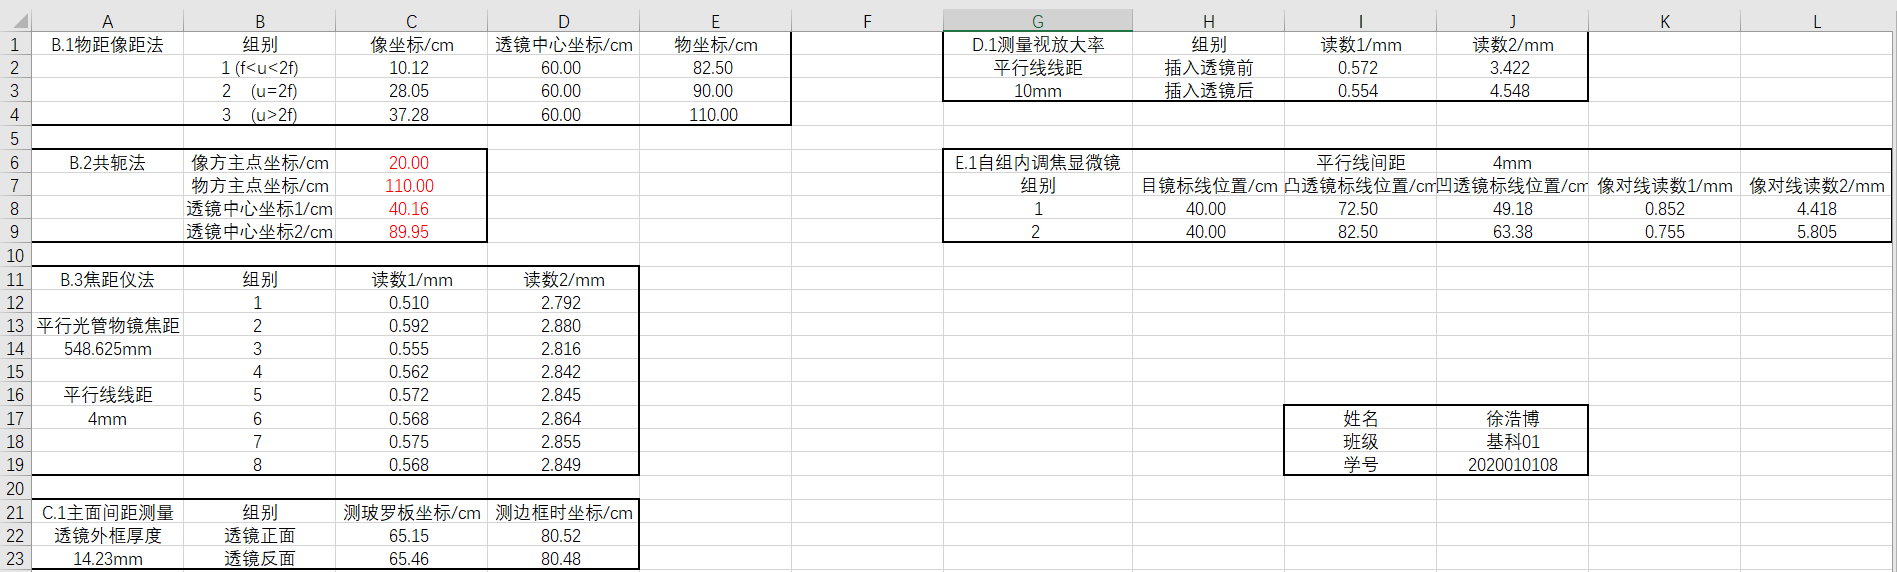
\includegraphics[scale=0.4]{data.PNG}
\end{center}\end{figure}
\vspace{2em}
\small{注:撰写报告过程中,我发现B.2部分的数据存在问题,并进行了重测,重测的数据已在截图中用红色标明. 由于值班老师无法采用拍照等方法进行数据留底,因此我请老师将我的情况告知于您. 给您带来了一定的打扰和不便,对此我向您表示抱歉!感谢您的理解.}
\end{document}

